\documentclass{article}
\usepackage{amsmath,graphicx,amssymb,amsthm,url}

\title{Implementation Assignment 4}
\date{\today}
\author{Rong Yu and Finn Womack}

\begin{document}
	\maketitle
	\section{K-Means}
	\subsection{Implementation}

After loading the data we ran it through our K-means algorithm. hen working with the larger data set this originally took about 50 iterations to converge but now takes about 5. The results of an iteration is displayed below:
	
	\begin{figure}[h!]
		\begin{center} 
			\includegraphics[scale=0.4]{kmeans.eps} 
		\end{center} 
		\label{fig:M1}
	\end{figure}
	

	\subsubsection{Visualization}
	
	Then just to look at the clusters we displayed random samples from each cluster. (running the algorithm with K = 4 this time) the results were as follows:
	
	\subsubsection*{Cluster 1}
	
	\begin{figure}[h!]
		\begin{center} 
			\includegraphics[scale=.6]{grp1.eps} 
		\end{center}  
		\label{fig:M2}
	\end{figure}
	
	\subsubsection*{Cluster 2}
	
	\begin{figure}[h!]
		\begin{center} 
			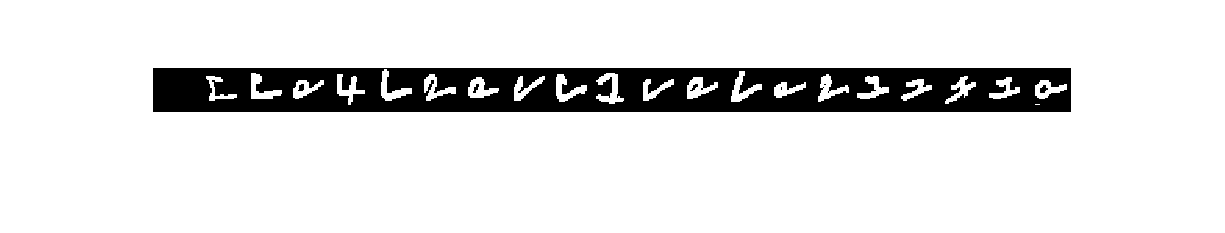
\includegraphics[scale=.6]{grp2.eps} 
		\end{center}  
		\label{fig:M3}
	\end{figure}
	
	\subsubsection*{Cluster 3}
	
	\begin{figure}[h!]
		\begin{center} 
			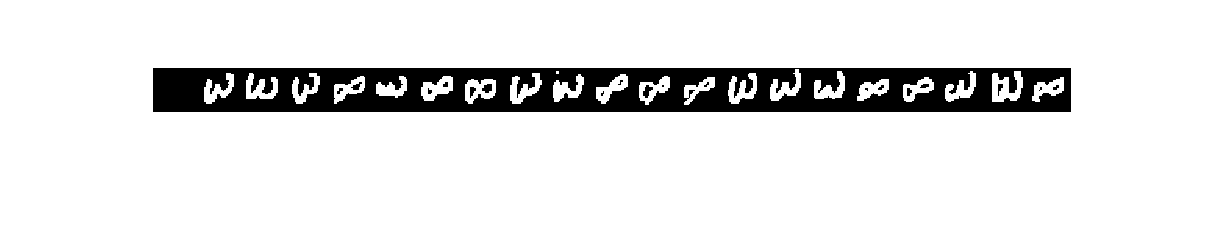
\includegraphics[scale=.6]{grp3.eps} 
		\end{center}  
		\label{fig:M4}
	\end{figure}
	
	\subsubsection*{Cluster 4}
	
	\begin{figure}[h!]
		\begin{center} 
			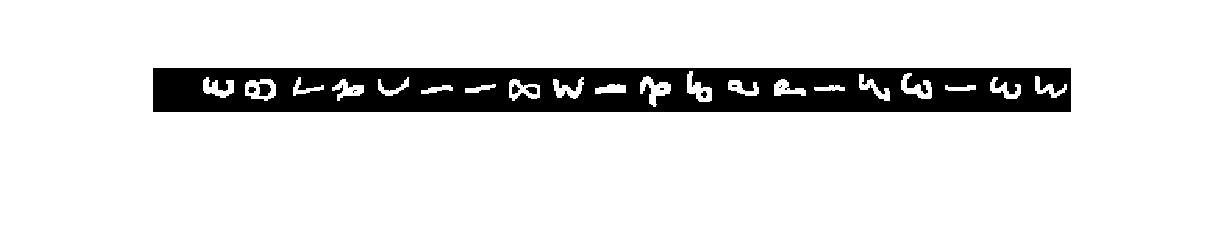
\includegraphics[scale=.6]{grp4.eps} 
		\end{center}  
		\label{fig:M5}
	\end{figure}
	
	\subsection{Different Ks}
	
	We then ran the algorithm on several different K values taking the minimum SSE of 10 iterations for each. We then plotted the values of k vs the values of the corresponding SSEs:
	
	\begin{figure}[h!]
		\begin{center} 
			\includegraphics[scale=0.4]{diffk.eps} 
		\end{center}  
		\label{fig:M6}
	\end{figure}
\newpage

Since the data set was reduced so much this figure doesn't really paint a clear picture as to which K values would work best. However, when we ran the algorithm on the larger data set \(not pictured because of how long it took\) We could see dramatic bends in the slope at K = 4 and K = 6. This implies that both might be good options and further investigation will be required to choose between the two. 

Upon inspection of the displays from last section it looks like K = 4 is combining 8s \& 3s as well as jumbling 1s, 7s, and 4s in a few clusters. Thus, we would likely pick 6 for the value of K.

\section{Hierarchical Agglomerative Clustering}
\subsection{Single Link}

We then implemented a single link algorithm. After running it we plotted a dendrogram for the last 10 clusters:
	
		\begin{figure}[h!]
		\begin{center} 
			\includegraphics[scale=0.4]{single.eps} 
		\end{center}  
		\label{fig:M7}
	\end{figure}
	
	It looks like the jumps in SSEs are small and slowing until we get to 6 clusters and then the SSE jumps up at 5 clusters and slightly start slowing again to until we have 1 cluster. Thus, from this dendrogram we would decide to go with 6 clusters. Also, as a side note, in this example we can really see the single links chaining effect. 
	
	\subsection{Complete Link}
	
	Lastly, we implemented a complete link algorithm. After running it we plotted a dendrogram for the last 10 clusters:
	
		\begin{figure}[h!]
		\begin{center} 
			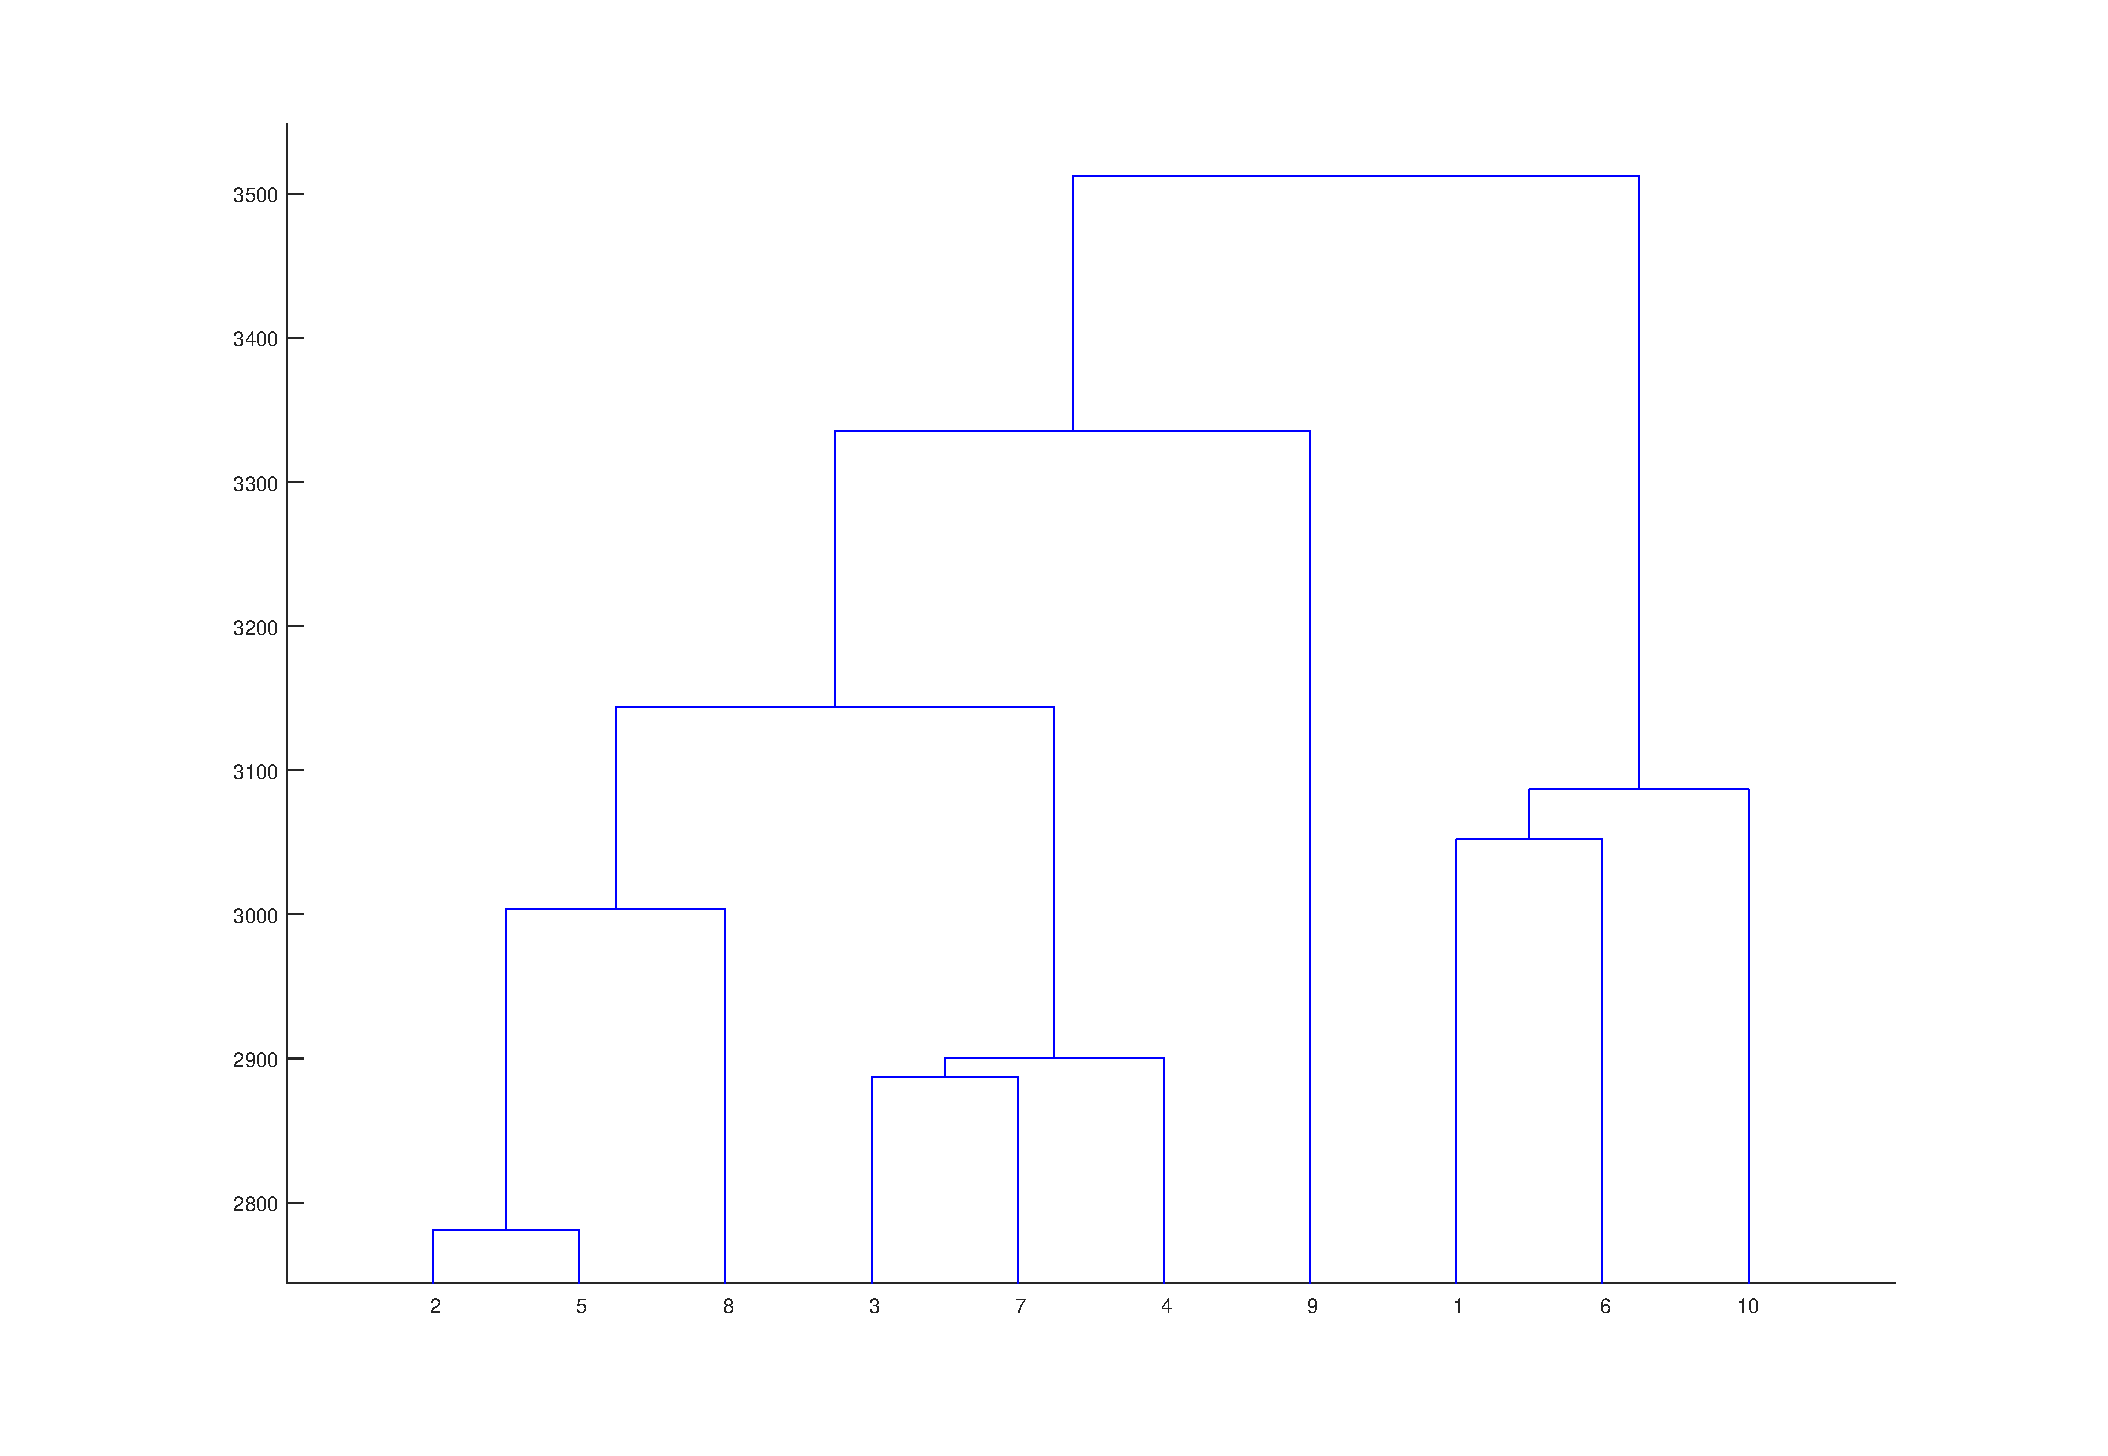
\includegraphics[scale=0.4]{complete.eps} 
		\end{center}  
		\label{fig:M8}
	\end{figure}
	
	From this it is harder to tell which number of clusters to choose. The biggest jump in SSE seems to happen when the clusters \{2, 5, 8, 3, 7, 4\} \& \{9\} merge. Before this there are 3 clusters, hence, we would likely decide that there are 3clusters from this dendrogram. 
	
	When compared to the other methods complete link seems to be the least apearant and reliable for this data set. We think that this is most likely due to the fact that the complete link method is sensitive to outliers.
	
	%\bibliography{myCitations} 
	%\bibliographystyle{abbrv}
	
\end{document} 